
\section{The Ski Jump}

Name \rule{2.0in}{0.1pt}\hfill{}Section \rule{1.0in}{0.1pt}\hfill{}Date \rule{1.0in}{0.1pt}

{\noindent \bf Objectives:} \begin{list}{$\bullet$}{\itemsep0pt \parsep0pt}

\item Introduce projectile motion \item Discover the angular dependence for trajectories

\end{list}

\noindent {\small {\bf Note:} The ski jump works by releasing the metal ball to roll down the channel and recording where it lands. For the purposes of laboratory exercise, the ball should be released from the same vertical height for all trials; use the horizontal support attached to the tall rod as a convenient reference point. The launch point is connected to a horizontal support attached to a short rod. This horizontal support rotates when you move the base of the tall rod nearer to or farther from the shorter rod. This rotation determines the angle at which the jump originates. The launching angle may be determined with a ruler and protractor by holding the ruler against the track in parallel with the launch point and then measuring the angle above the horizontal with the protractor (see figure below).}

\vspace{0.3cm}
{\par\centering 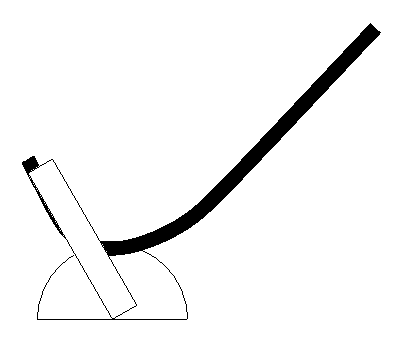
\includegraphics{ski_jump_fig1.eps} \par}
\vspace{0.3cm}

{\noindent \bf Apparatus:} \begin{list}{$\bullet$}{\itemsep0pt \parsep0pt}

\item jump chute \item metal ball \item protractor and ruler \item two wooden boards \item sheets of white and carbon paper

\end{list}

{\noindent \bf Activity:} \begin{enumerate}

\item  Set up the jump and landing surface so that the launch point and landing surface are at the same height.

\item  With the benefit of several trial runs at different angles, decide where you should tape a piece of white paper down so all jumps will land on the paper. Cover the paper with a piece of carbon paper, ink side down.

\item  Attempt several jumps each at a number of different angles, say 20, 30, 37, 45, 53, 60, and 70 degrees. Circle the impact points for a given angle and label them before proceeding to the next angle.

\item  Note the relative ranges of the ball's flight as a function of the launching angle: \vskip35pt

\end{enumerate}

\pagebreak

\textbf{Questions:}

\begin{enumerate}
\item Is the range always the same, or does it depend on the angle? Describe the dependence,
if any. \vspace{20mm}

\item At which angle is the range a maximum?\vspace{10mm}

\item How are the ranges and angles related on either side of the maximum?\vspace{20mm}

\item How do you think this angular dependence would change for landing surfaces at
different heights? Test your predictions.
\end{enumerate}
